\documentclass[11pt]{article}
\input{\string~/.macros}
\usepackage[a4paper, total={7in, 9in}]{geometry}
\usepackage{bbm}
\usepackage{mathrsfs} % really cursive alphabets
\usepackage{graphicx}
    \graphicspath{{./assets}}
\usepackage{hyperref}
    \hypersetup{colorlinks=true, linktoc=all, linkcolor=blue, citecolor=red}
\usepackage[backend=bibtex,sorting=none]{biblatex}
\usepackage[margin=0cm]{caption}

% random variables
\newcommand\ry{\ensuremath{\mathsf{y}}}
\newcommand\rx{\ensuremath{\mathsf{x}}}
\newcommand\rb{\ensuremath{\mathsf{b}}} 
\newcommand\rc{\ensuremath{\mathsf{c}}}
\newcommand\rz{\ensuremath{\mathsf{z}}}
\newcommand\ru{\ensuremath{\mathsf{u}}}
\newcommand\rw{\ensuremath{\mathsf{w}}}
\newcommand\rpa{\ensuremath{\mathsf{pa}}}
\newcommand\rU{\ensuremath{\mathsf{U}}}
\newcommand\rbx{\ensuremath{\mathsf{\mathbf{x}}}}
\newcommand\rby{\ensuremath{\mathsf{\mathbf{y}}}}
\newcommand\rbu{\ensuremath{\mathsf{\mathbf{u}}}}

\newcommand\bbP{\ensuremath{\mathbbm{P}}}
\newcommand\bbQ{\ensuremath{\mathbbm{Q}}}


% boldsymbols
\renewcommand\bmu{\ensuremath{\boldsymbol{\mu}}}
\newcommand\bSigma{\ensuremath{\boldsymbol{\Sigma}}}
\newcommand\bgamma{\ensuremath{\boldsymbol{\gamma}}}
\newcommand\bomega{\ensuremath{\boldsymbol{\omega}}}
\newcommand\bnu{\ensuremath{\boldsymbol{\nu}}}


% optimization, classes of functions
\newcommand\scrF{\ensuremath{\mathscr{F}}}
\newcommand\scrS{\ensuremath{\mathscr{S}}}
\newcommand\scrP{\ensuremath{\mathscr{P}}}

% independence
\newcommand{\dperp}{\ensuremath{\perp\!\!\!\perp}}
\newcommand{\ndperp}{\ensuremath{\not\!\perp\!\!\!\perp}}

% operators
\newcommand{\prox}{\ensuremath{\mathsf{prox}}}
\addbibresource{GP.bib}
\addbibresource{multitask.bib}


\begin{document}
 
\section{Gaussian Process}

\cite{carledwardrasmussenGaussianProcessMachine2006} introduces Gaussian Process regression as an alternative view to Bayesian regression. 

\subsection{Bayesian Regression}
 
In linear regression setup, we assume output $y\in\R$ is a linear function of inputs $x\in\R^d$, corrupted with additive iid normal noise,
\begin{align}
    y = f(x) + \epsilon
    \quad\text{where}\quad
    f(x) = w^Tx
    \quad\text{and}\quad
    \epsilon \sim \sN(0, \sigma_n^2)
\end{align}
The Bayesian setup considers $w\in\R^d$ as a random variable, endowed with prior $w\sim \sN(0,\Sigma_p)$. Using Bayes rule, we can find the posterior of weights given data, which is again a normal random variable $p(w \mid X, y) = \sN\left(w \; ; A^{-1}b, A^{-1} \right)$ where $A=\frac{1}{\sigma_n^2} X^TX + \Sigma_p^{-1}$ and $b = \frac{1}{\sigma_n^2}X^Ty$ and $X\in\R^{n\times d}, y\in\R^{n\times 1}$ are design matrices. For test point $x_*$, the predictive distribution of $f_*=f(x_*)$ is the average likelihood of $f_*$ under model $f(x;w)$ with respect to posterior of $w$.
\begin{align}
    p(f_*\mid x_*, X, y)
        = \int p(f_*\mid x_*,w) p(w\mid X, y) \, dw
    \label{eq:kernel_bayesian_regression_predictive_distribution_integral}
\end{align}
We can think of the predictive distribution as a linear function $f_* = x_*^Tw$ of weights, a normal random variable, and therefore is normal. Therefore, $f_*\mid x_*,X,y \sim \sN( x_*^T A^{-1}b, x_*^T A^{-1}x_* )$. The natural extension to Bayesian linear regression is to kernelize it, for example assume a linear model in some feature space $f(x) = \phi(x)^Tw$ for some feature map $\phi:\R^d\to\R^D$. We can write predictive distribution as 
\begin{align}
    f_* \mid x_*,X,y \sim \sN(
        & k(x_*,X) (k(X,X)+\sigma_n^2 I)^{-1}y, \\
        & k(x_*,x_*) - k(x_*,X)(k(X,X) + \sigma_n^2 I)^{-1} k(X,x_*))
    \label{eq:kernel_bayesian_regression_predictive_distribution}
\end{align}
where $k(X,X') = \Phi \Sigma_p \Phi'^T \in \R^{n\times n'}$ and $\Phi\in\R^{n\times D}$ are the feature vectors.

\subsection{Gaussian Process}


\begin{definition}
    (Gaussian Process) A Gaussian process is a stochastic process $\pc{X_t}_{t\in T}$ such that, for every finite subset of indices $t_1,\cdots,t_k \in T$, $(X_{t_1},\cdots,X_{t_k})$ is multivariate normal.
\end{definition}

A Gaussian process $f\sim \sG\sP(m,k)$ over $\R^{\sX}$ is fully specified by the mean function $m:\sX\to\R$ and covariance function $k:\sX\times\sX\to\R$ where
\begin{align}
    m(x)=\E\pb{f(x)}
    \quad\quad\quad
    k(x,x') = \E\pb{ (f(x)-m(x))(f(x')-m(x')) }
\end{align}
The covariance function determines function's behavior, for example its stationarity, smoothness, and periodicity etc. For example, the squared exponential covariance function $k_{\text{SE}}(x,x') = \exp( -\frac{1}{2\ell^2} \norm{x-x'}_2^2 )$ enforces the prior knowledge that functions are smooth, i.e. inputs are close in the Euclidean sense will have similar outputs. See Figure (\ref{fig:plt_sample_from_gp}) for some examples of samples from Gaussian process.

\begin{example}
    (Intuition about covariance matrix for $\sG\sP$) First consider $(y_1,y_2) \sim \sN(\mathbf{0}, \Sigma)$ where $\Sigma_{11}=\Sigma_{22} = 1$ and $\Sigma_{12}=\Sigma_{21}=\rho_{12}$. We know $y_1\mid y_2 = a \sim \sN(\rho_{12} a, 1 -  \rho_{12}^2)$. When $\cov(y_1,y_2) = \rho_{12} \uparrow 1$, $y_1$'s samples conditioned on $y_2=a$ fall close to $a$ with high probability. When $\rho_{12} \downarrow 0$, $y_1 \mid y_2=a$ will distribute like a unit normal, regardless of values that $y_2$ take. Extend this intuition to gaussian process: whenever $k(x_i,x_j)$ is large, $y_i,y_j$ are correlated and so observing $y_i=a$ provides a strong prior on how $y_j$ will behave, or in other words, reduce the uncertainty of values that $y_j$ can take dramatically.
\end{example}


\begin{center} 
\begin{figure}[h!]
    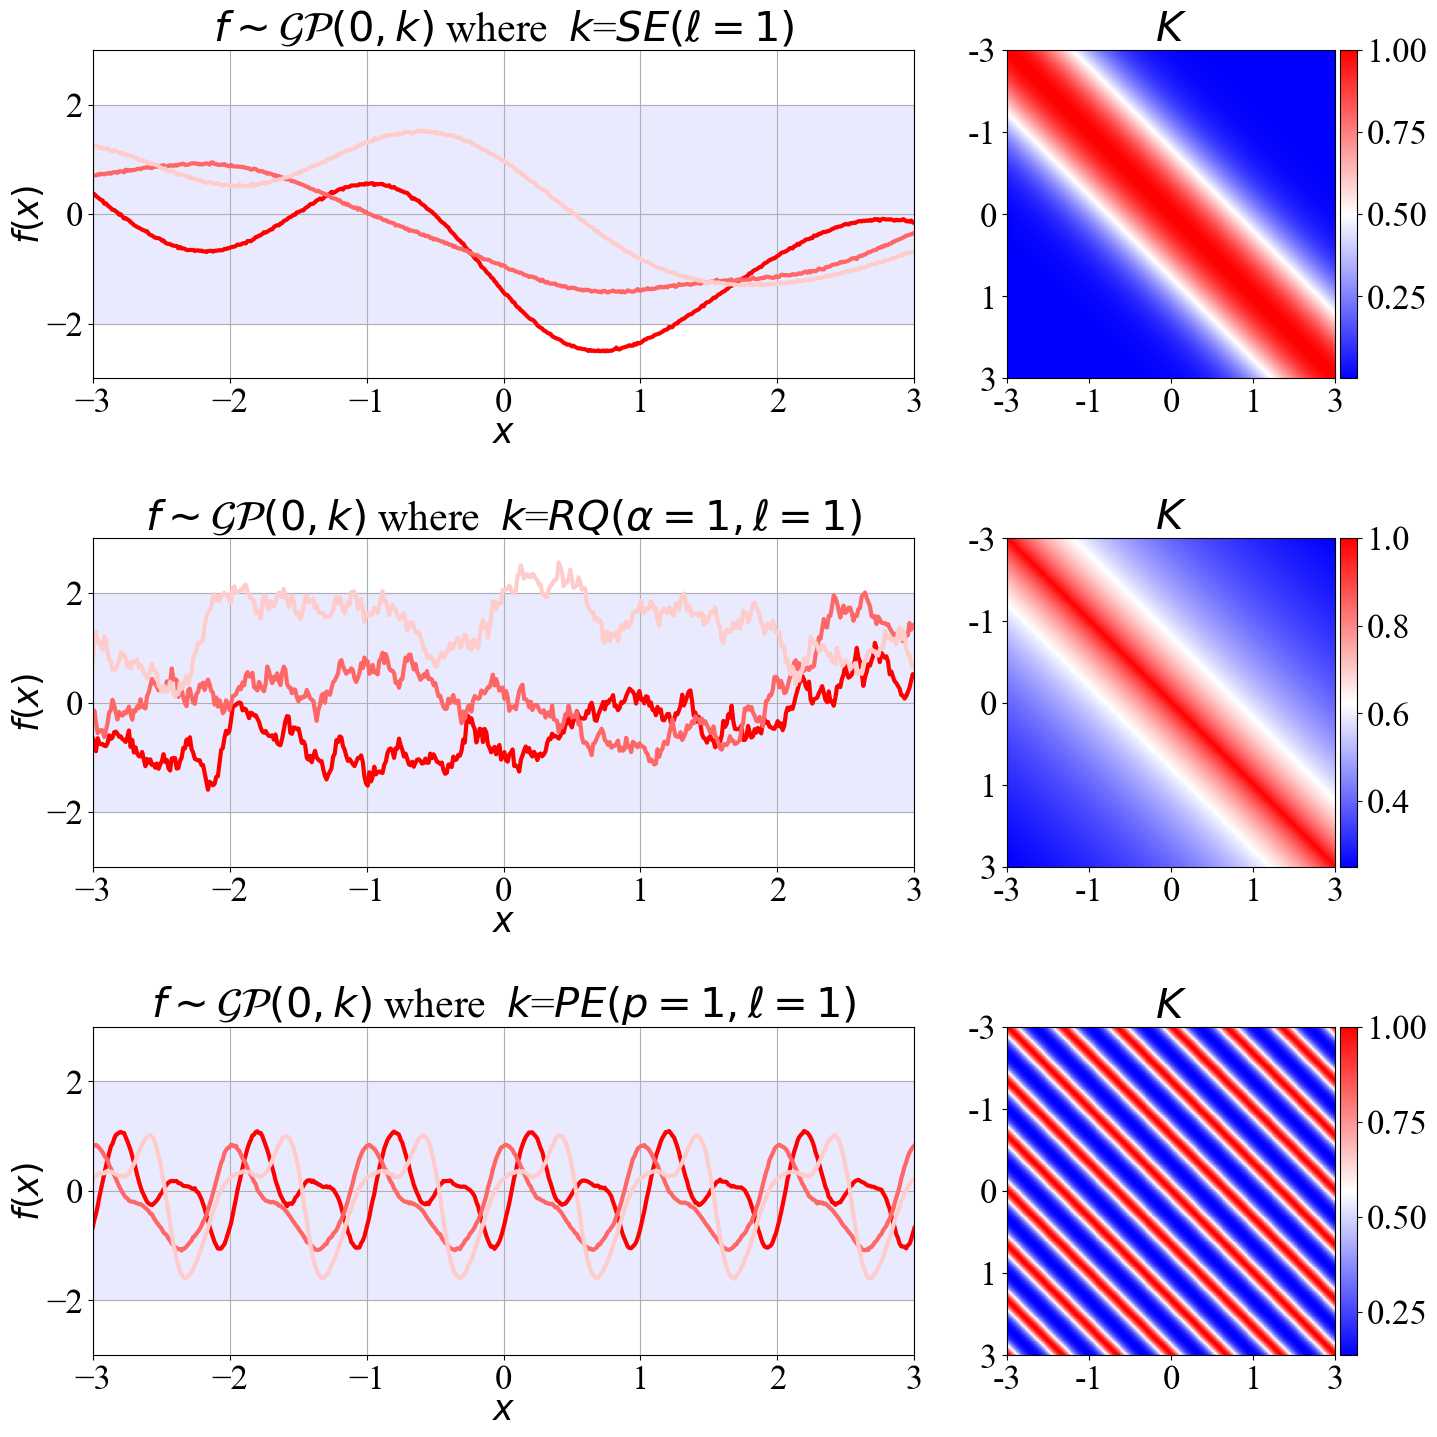
\includegraphics[width=\textwidth]{assets/plt_sample_from_gp.png} 
    \caption{(Left) Samples from Gaussian process prior and (Right) covariance matrix at test locations.}
    \label{fig:plt_sample_from_gp}
\end{figure}
\end{center} 
    

\subsection{Gaussian Process Regression}

Instead of placing a prior over weights $p(w)$ to quantify randomness in function $f(x)=\phi(x)^Tw$, we model function directly as a Gaussian process, $f\sim \sG\sP(0,k)$. There is a one-to-one correspondence between the two views. For example, $f(x)=\phi(x)^Tw$ with prior $w\sim \sN(0,\Sigma_p)$ used in kernel Bayesian regression has
\begin{align}
    \E\pb{f(x)}
        = \phi(x)^T \E\pb{w} = 0
    \quad\quad\quad
    \E\pb{ f(x)f(x') }
        = \phi(x)^T\Sigma_p \phi(x')
\end{align}
Therefore, $f\sim \sG\sP(0, k)$ where $k(x,x') = \phi(x)^T \Sigma_p \phi(x')$. Note $k$ is in fact a valid kernel. (Since $\Sigma_p$ is psd, $\Sigma_p = UDU^T$ by SVD. We can write $k(x,x') = \inner{\psi(x)}{\psi(x')}$ where $\psi(x) = \Sigma_p^{1/2} \phi(x)$ and $\Sigma_p^{1/2} = UD^{1/2}U^T$). Conversely, any valid kernel used in kernel Bayesian regression can be used to parameterize the covariance function of the Gaussian process model over $f$.

Since $y=f(x)+\epsilon$, we have $\by = \mathbf{f} + \sigma_n^2 I \sim \sN(0, k(X,X)+\sigma_n^2I)$ where $\by,\mathbf{f}\in\R^{n\times 1}$. We can write the joint distribution of observed values and function values at some test locations $X_*$ as
\begin{align}
    \begin{bmatrix}
        \by \\ \mathbf{f}_*
    \end{bmatrix}
    \sim
    \sN\left(
        \mathbf{0},
        \begin{bmatrix}
            k(X,X) + \sigma_n^2I & k(X,X_*) \\
            k(X_*,X) & k(X_*,X_*) \\ 
        \end{bmatrix}
    \right)
    \label{eq:gaussian_process_regression_noisy_model}
\end{align}
We can derive the predictive distribution for $\mathbf{f}_*\mid \by$ by simply apply conditional distribution formula
\begin{align}
    \mathbf{f}_* \mid X,\by, X_* \sim \sN(
        & k(X_*,X) (k(X,X)+\sigma_n^2 I)^{-1} \by  \\
        & k(X_*,X_*) - k(X_*,X) (k(X,X)+\sigma_n^2 I)^{-1} k(X,X_*) )
    \label{eq:gp_regression_predictive_distribution}
\end{align}
which has exact form compared to (\ref{eq:kernel_bayesian_regression_predictive_distribution}). More compactly, for a single test point $x_*$, $\mu_{\mathbf{f}_*} =  k_*^T (K+\sigma_n^2 I)^{-1}$ and $\var(\mathbf{f}_*) = k(x_*,x_*) - k_*^T (K+\sigma_n^2 I)^{-1} k_* $ where $k_* = k(X,x_*)\in \R^{n\times 1}$. See Figure (\ref{fig:plt_gp_regression_inference}) for examples of Gaussian process regression with varying data size and hyperparameters. 


\begin{center} 
\begin{figure}[h!]
    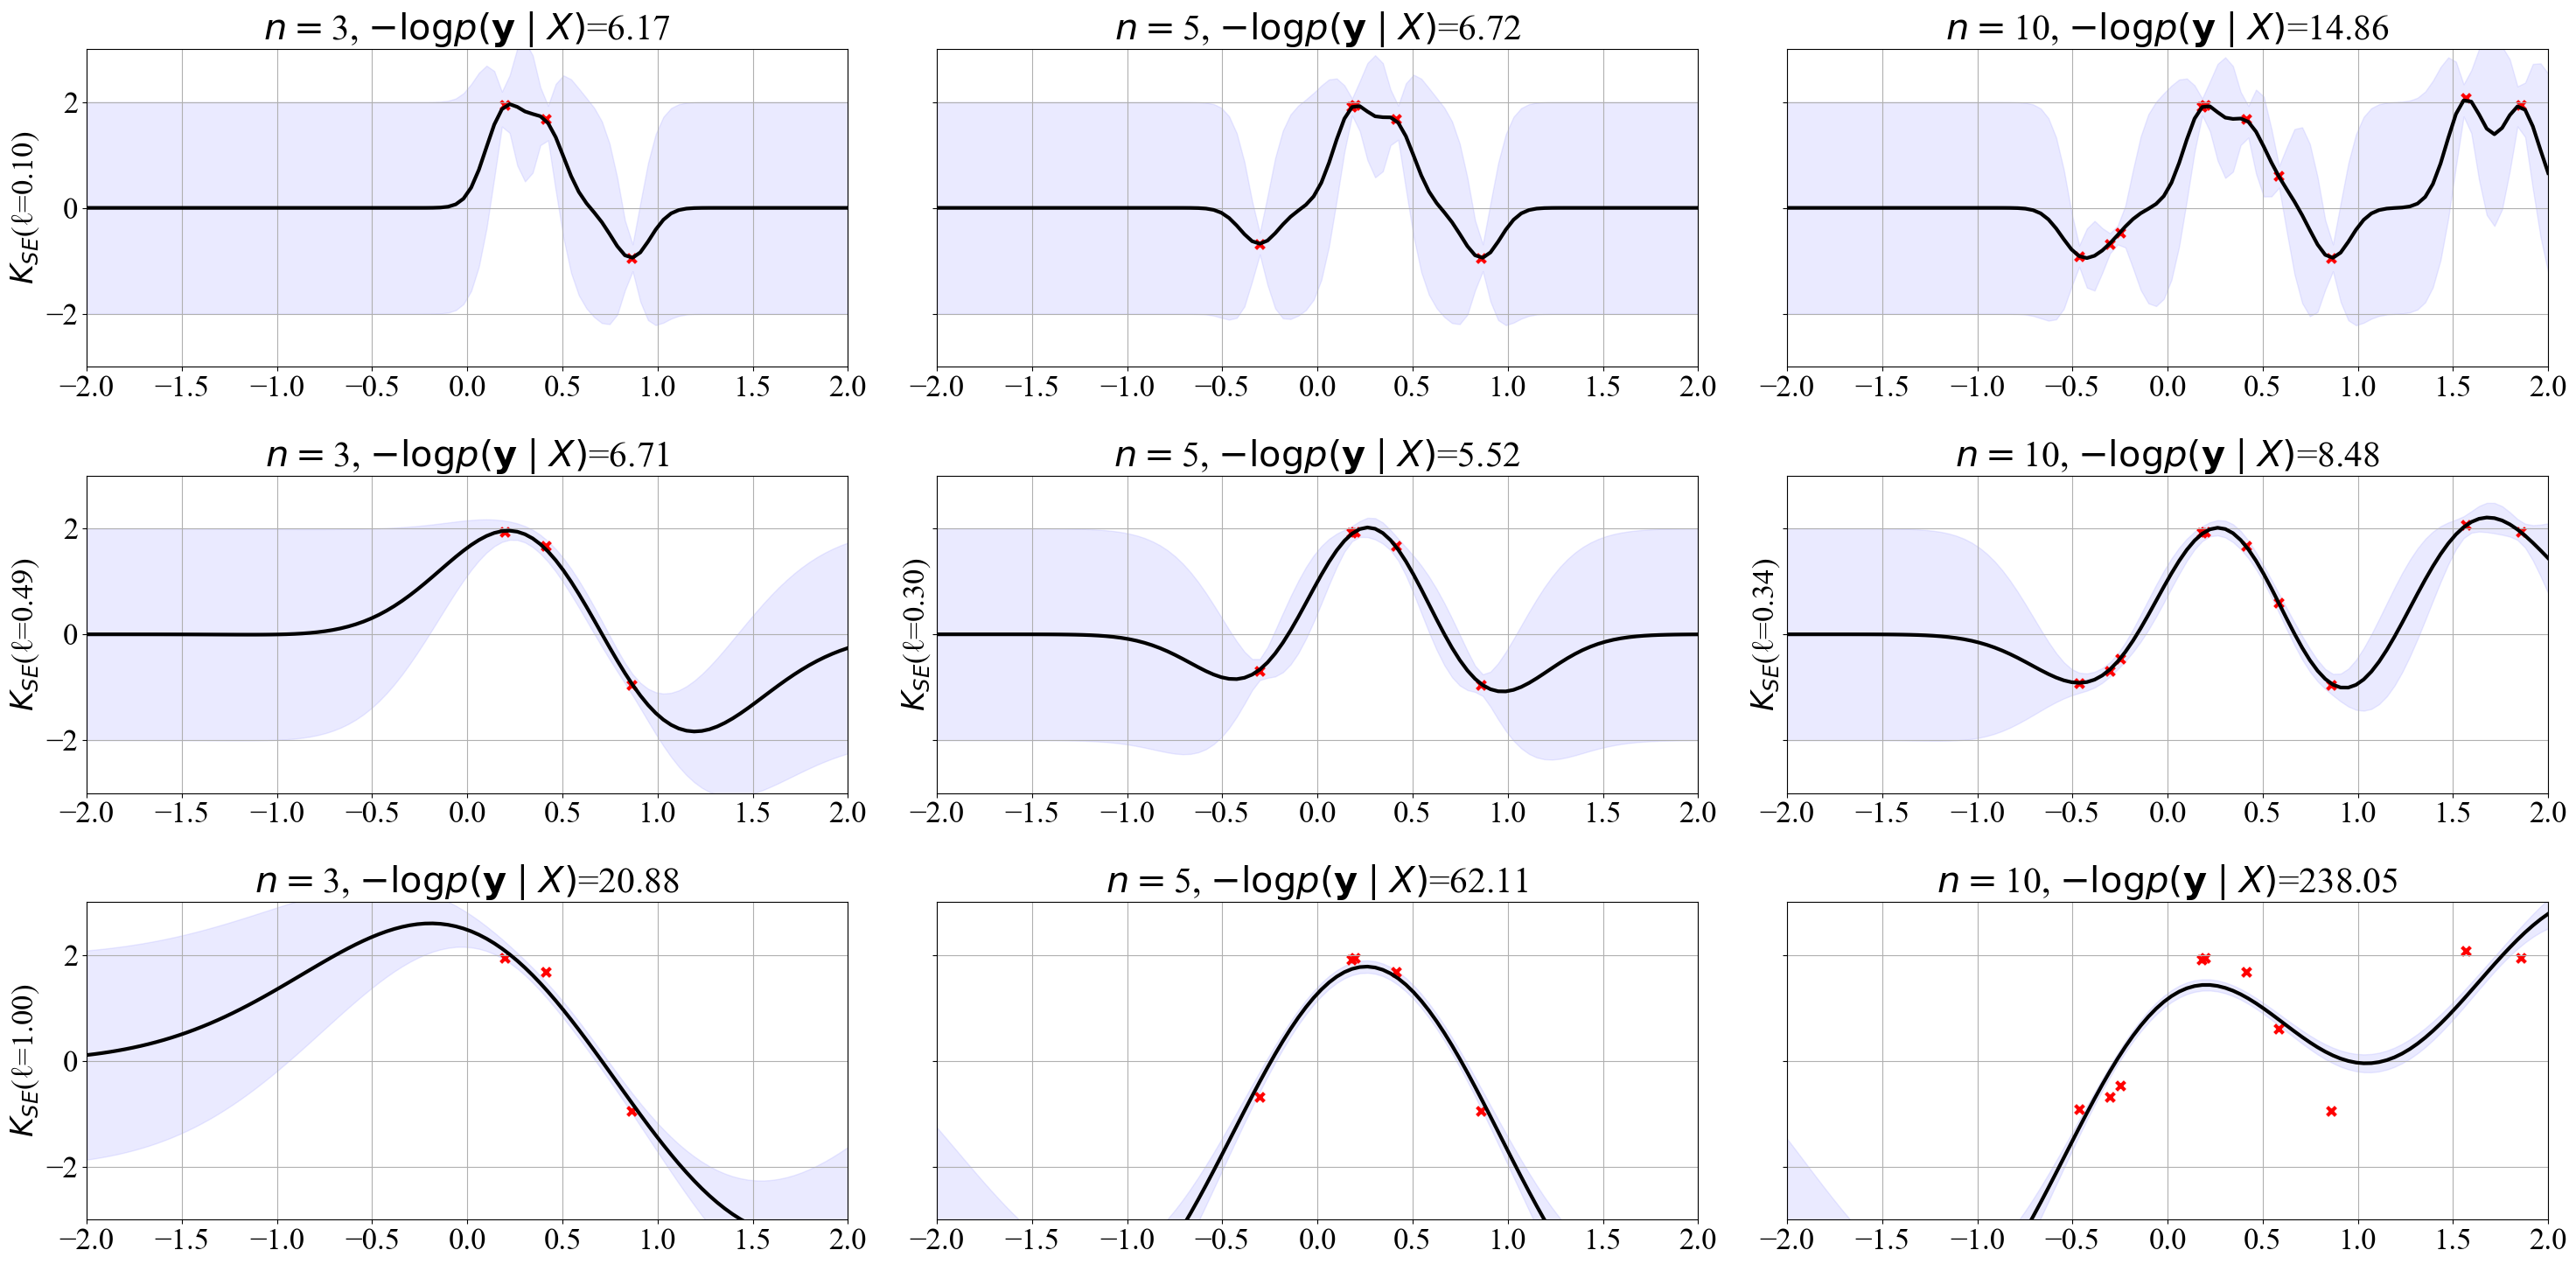
\includegraphics[width=\textwidth]{assets/plt_gp_regression_inference.png} 
    \caption{This plot shows mean (black) and 95\% confidence interval (light blue) for predictive distribution $p(\mathbf{f}_*\mid X,\by, X_*)$ fit using Gaussian process regression assuming a SE prior over $f\sim\sG\sP(0,k_{SE})$ of varying lengthscale $\ell$ and observed sample sizes $n$. The middle row's kernel hyperparameter is taken to be the empirical Bayes estimate $\ell = \argmax p(\by\mid X, \ell)$ where $p(\by\mid X,\ell)$ given by Equation (\ref{eq:gp_regression_marginal_likelihood}), optimized via gradient descent. Here the we cheat by providing the groundtruth noise $\sigma_n=.1$. Optimizing for $\pc{\ell,\sigma_n}$ is hard and prone to local minima.}
    \label{fig:plt_gp_regression_inference}
\end{figure}
\end{center}

\subsection{Model Selection}

Model selection for Gaussian process regression involves picking the form and the hyperparameters of the covariance function. Given data $(X,\by)$, marginal likelihood $p(\by\mid X)$ quantifies how likely data is observed under our additive noise model $\by\mid \mathbf{f} \sim \sN(\mathbf{f},\sigma_n^2 I)$ on average with respect to latent function values (or parameters of our model) $\mathbf{f}\mid X \sim \sN(0,K)$ (due to assumption of Gaussian process prior over f),
\begin{align}
    p(\by\mid X)
        = \int p(\by\mid \mathbf{f},X) p(\mathbf{f}\mid X) \, d\mathbf{f}
\end{align}
This formulation is analogous to that in Bayesian linear regression where the marginal likelihood marginalizes over weights $p(\by\mid X) = \int p(\by\mid X,w)p(w) \, dw$. We can obtain a closed form expression by reading off (\ref{eq:gaussian_process_regression_noisy_model}), i.e. $\by \sim \sN(\mathbf{0}, K+\sigma_n^2 I)$. 
\begin{align}
    \log p(\by\mid X)
        = -\frac{1}{2} \by^T  (K+\sigma_n^2 I)^{-1}\by - \frac{1}{2} \log |K+\sigma_n^2I| - \frac{n}{2} \log 2\pi 
    \label{eq:gp_regression_marginal_likelihood}
\end{align}
In Bayesian model selection, model hyperparameters for Gaussian process regression $\theta = \pc{\sigma_n, \ell}$ can be found by maximizing the marginal likelihood or the type II likelihood $\theta^* = \argmax_{\theta}\, \log p(\by\mid X, \theta)$.



\section{Multitask Learning}

\subsection{MTGP}

Multitask Gaussian Process (MTGP) regression \cite{bonillaMultitaskGaussianProcess2008} is a method to do multitask learning using Gaussian process. Given design $X\in\R^{N\times D}, Y\in\R^{N\times M}$, we want to learn a vector valued regressor $f:\R^D\to\R^M$ that fits data well. We can put a GP prior over $f \sim \sG\sP(0,k)$ where the covariance function models both the relationship between inputs via $k_x$ and similarity between tasks / output coordinate via $k_t$, specifically define $k$ as tensor product $k_x\otimes k_t$ over $\sX\times\sT$ where $\sT = \pc{1,2,\cdots,M}$ is space of tasks,
\begin{align}
    k((x,t),(x',t')) = k_x(x,x')\; k_t(t,t')
\end{align}
Consider a likelihood model with task specific noise variance $y_t \sim \sN( f_t(x), \sigma_t^2 )$. Denote $Y_t$ as $t$-th column in $Y$, then $Y_t \sim \sN( 0,  k_t(t,t) K + \sigma_t^2 I )$ where $\pb{K}_{ij} = k_x(x_i,x_j)$. Furthermore, if we let $\by = \text{vec}(Y) = (Y_1,\cdots,Y_M)$, then $\by \sim \sN(0,\Sigma)$ where
\begin{align}
    \Sigma = 
    K^t \otimes K + D \otimes I
    = 
    \begin{bmatrix}
        K^t_{11} K + \sigma_1^2 I & K^t_{12} K & \cdots & K^t_{1M} K \\ 
        K^t_{21} K & K^t_{22}K + \sigma_2^2 I & \cdots & K^t_{2M} K \\ 
        \vdots & \vdots & \ddots & \vdots \\
        K^t_{M1} K & K^t_{M2}K  & \cdots & K^t_{MM} K + \sigma_M^2 I \\
    \end{bmatrix}
\end{align}
The task similarity matrix $K_t$ ($\pb{K_t}_{ij} = k_t(i,j)$) induce correlation between tasks. Intuitively, if two tasks $t,t'$ are related in the sense an optimal regressor for $y_t,y_{t'}$ vary together in some systematic manner, then observation at some location $(x,y_t)$ constrains what the value $y_{t'}$ can take. The degree to which we can reduce the uncertainty that $y_{t'}$ can takes depends on $k_t(t,t')$. Therefore, a learner which utilizes information obtained from related tasks can be learnt more efficiently than if learnt without knowledge of other tasks, in which case $K_t = I$. \cite{bonillaMultitaskGaussianProcess2008} proposes to use EM to first impute missing latent variables $\mathbf{f}$ from noisy observations $\by$, then find hyperparameters $\theta = \pc{ \theta_{k_x}, K^t }$ by maximizing the full data likelihoods $p(\by,\mathbf{f} \mid \theta_{k})$. Alternatively, we can simply can learn the hyperparameters by applying gradient descent to maximize type-II likelihood $\theta^* = \argmax_{\theta} \log p(\by\mid X, \theta)$.

\subsection{Asymmetric MTGP}

When the goal is to improve performance of a target/main task given the other tasks, optimizing for maximum marginal likelihood of all tasks is suboptimal. 

There are extension of MTGP to the asymmetric case by assuming that auxiliary task functions are addition of a shared main task function and task specific function \cite{leenFocusedMultitaskLearning2012}, however it still uses the full marginal likelihood for all tasks to find task similarity and kernel hyperparameters. Ideally, we want
\begin{enumerate}
    \item An objective which depends on likelihood of main task only
    \item Automatically learn the task similarity such that auxiliary task or side information can improve learning of main task. If a side task is totally unrelated to the main task, it should have minimal influence on learning of the main task.
\end{enumerate}


 


\newpage
\printbibliography 




\end{document}